\chapter{Background}
\label{ch:background}
In this chapter, we will describe how we approached problems of trust in global peer-to-peer environment in section \ref{sec:computational-model},how can we evaluate single interaction between two peers in section \ref{sec:interaction-evaluation-strategies}, how we mitigate cold start problem \ref{sec:cold-start-problem} and finally, how do we aggregate network threat intelligence into a single network opinion in section \ref{sec:network-intelligence-aggregation}.

Our trust model, Fides, operates in four phases, first it receives data, then it aggregates the data, evaluates the interactions with each peer and as a last step it updates the service trust for the next interaction.
See figure \ref{fig:trust-model-life-cycle}, where is this process visualized.

\begin{figure}[ht!]
    \centering
    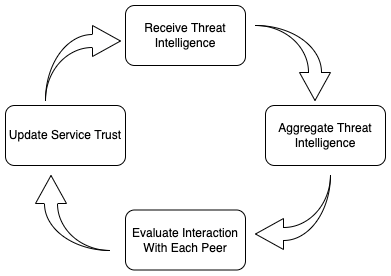
\includegraphics[width=0.7\textwidth]{assets/service_trust_diagram.png}
    \caption{Trust Model Life Cycle}
    \label{fig:trust-model-life-cycle}
\end{figure}

In the following sections we will be using following terminology and words when talking about the trust model.

\begin{itemize}
\item \textbf{Fides} - name of the trust model, performs all trust related computations
\item \textbf{service trust} - how much a trust model trust a peer to provide us a good service - it is not necessarily how much we trust the data we received from the peer as to the final computation we may include the information about peer's IP address from the Slips (what does Slips think about the IP address)
\item \textbf{target} - an IP address or domain - point of interest that can be source of network traffic and Slips has a capability to assign threat intelligence data to this object
\item \textbf{remote peer} - peer that is running somewhere on the internet and it is connected to the global peer-to-peer network
\item \textbf{local peer} - local instance of Slips that is connected to the global peer-to-peer network and runs instance of Fides
\end{itemize}

\section{Computational Model of Fides}
\label{sec:computational-model}
This section describes how does Fides come up with a single most important value $st_{i,j}$ service trust. Service trust describes how much can local peer $i$ trust remote peer $j$.
Used algorithm, or in other words the trust model itself, that computes $st_{i,j}$, is based on SORT\cite{sort} with modifications to fit our use case - a global peer-to-peer network for sharing threat intelligence. 
The modifications are based on the interaction evaluation strategies proposed in \ref{sec:interaction-evaluation-strategies} and algorithms to solve cold start problem described in \ref{sec:cold-start-problem}. 
The table \ref{tab:notation-computational-model} describes the most important notation we use in the following sections.

\begin{table}[ht]
\centering
\begin{tabular}{ c | m{20em} }
 $i$ & local peer, instance of Fides \\
 \hline
 $j$ & remote peer somewhere on the internet \\
 \hline
 $st_{i, j}$ & service trust - how much $i$ trusts $j$ that it provides good service \\
 \hline
 $r_{i, j}$ & $i$'s reputation value about $j$ \\
 \hline
 $rt_{i, j}$ & $i$'s recommendation trust about $j$ \\
 \hline
 $sh_{i, j}$ & size of $i$'s service history with $j$ \\
 \hline
 $s^{k}_{i, j}$ & $i$'s satisfaction value with interaction with peer $j$ in window $k$\\
 \hline
 $w^{k}_{i, j}$ & weight of $i$'s interaction with $j$ in $k$ \\
 \hline
 $f^{k}_{i, j}$ & fading effect of $i$'s interaction with $j$ in $k$ \\
\end{tabular}
\caption{Fides Computational Model Notation}
\label{tab:notation-computational-model}
\end{table}

\subsection{Intuition}
In the following pages, we describe the process top-down starting with the most important parts - service trust - and then breaking it down to bits.
There are two main ideas behind the most of the equations. 

The first one is that we want to robustly capture average behavior of the peers. In order to do that, we will be computing average behavior and standard deviations from said behavior and normalizing them.

Secondly, we will be comparing and weighting first hand experience with the remote experience. 
First hand experience is what happened between local and remote peer during time they interacted. This can be, for example, threat intelligence sharing, file sharing or the results of recommendation protocol.
Remote experience is what happened between one remote peer and another remote peer. In other words, first hand experience for peer $j$ are actions between $j$ and $z$. When $j$ shares information about these action with peer $i$, for $i$ it is a remote experience.

\subsection{Service Trust}
\label{subsec:service-trust}
One of the major goals of the algorithm is to compute the service trust $st_{i,j}$. 
Service trust is a value that describes how much does peer $i$ trust remote peer $j$, that it is going to provide \textit{good service}.
We compute the value by weighting local experience with peer's $j$ service, with the reputation $j$ got from the network, when it was first seen by $i$.
The used weight is the size of the service interaction history $sh_{i,j}$ to maximal history size $sh_{max}$.

\begin{equation}
\label{eq:service-trust}
    st_{i,j}=\frac{sh_{i,j}}{sh_{max}} \cdot \left(cb_{i,j} - \frac{1}{2} ib_{i,j} \right) +\left(1-\frac{sh_{i,j}}{sh_{max}}\right) \cdot r_{i,j}
\end{equation}

The service trust equation (\ref{eq:service-trust}) implies that the more interaction there was, between $i$ and $j$, the bigger impact on $st_{i,j}$ it has. 
In other words, the more $i$ and $j$ interact the less $i$ rely on the reputation, that $i$ computed from the values provided by the network, at the time when $j$ was seen for the first time and it 

\subsection{Local Experience for Service Trust}
First part of the equation \ref{eq:service-trust} contains \textit{competence belief}, $cb_{i,j}$, and $ib_{i,j}$ - \textit{integrity belief}.
Both of the values are based solely on the interactions history that peer $i$ experienced with the peer $j$.

\subsubsection{Competence Belief}
\textit{Competence belief} represents how much did peer $j$ satisfy local peer $i$ with the past interactions. We measure it as an average of interactions from the past \cite{sort}.
\begin{equation}
\begin{split}
    cb_{i,j} &= \frac{1}{\beta_{cb}} \sum_{k=1}^{sh_{i, j}} s_{i,j}^{k} \cdot w_{i,j}^{k} \cdot f_{i,j}^{k} \\
    \beta_{cb} &= \sum_{k=1}^{sh_{i, j}} s_{i,j}^{k} \cdot w_{i,j}^{k}
\end{split}
\end{equation}
It holds that $0 \leq cb_{i,j} \leq 1$ and where $s^{k}_{i,j}$ is the evaluation of the interaction in window $k$, $w^{k}_{i, j}$ is the weight of the interaction (how important it was) and $f^{k}_{i,j}$ is the fading effect of that interaction. We describe $s^{k}_{i,j}$, $w^{k}_{i,j}$ and $f^{k}_{i,j}$ in greater detail in \ref{subsec:evaluating-an-interaction}. 
$\beta_{cb}$ is the normalization coefficient that ensures that $cb_{i, j}$ stays within the interval of $0 \leq cb_{i,j} \leq 1$.

\subsubsection{Integrity Belief}
\textit{Integrity belief} is a level of confidence in predictability of future interactions. $ib_{i,j}$ is then measured as deviation from the average behavior $cb_{i,j}$. 
Therefore, $ib_{i,j}$ is calculated as an approximation to the standard deviation of interaction parameters\cite{sort}.
\begin{equation}
\begin{split}
    ib_{i,j} &= \sqrt{\frac{1}{sh_{i,j}} \sum_{k=1}^{sh_{i,j}}\left(s_{i,j}^{k} \cdot w_{i,j}^{\mu} \cdot f_{i,j}^{\mu} - cb_{i,j}\right)^{2}} \\
    f_{i,j}^{\mu} &= \frac{1}{sh_{i, j}} \sum_{k=1}^{sh_{i,j}} f^{k}_{i,j} \\
    w_{i,j}^{\mu} &= \frac{1}{sh_{i, j}} \sum_{k=1}^{sh_{i,j}} w^{k}_{i,j}
\end{split}
\end{equation}

It holds that $0 \leq ib_{i,j} \leq 1$.
The more consistent behavior peer $j$ has, the lower the $ib_{i,j}$ is. Consistency is highly desired property as the local peer then have more precise estimates about future behavior of the remote peer.

\subsection{Evaluating an Interaction}
\label{subsec:evaluating-an-interaction}
\todo{Should we keep it here or move somewhere else?}
In section \ref{sec:interaction-evaluation-strategies}, we describe multiple strategies in detail, how to compute $s^{k}_{i,j}$ - satisfaction value with $k$th interaction of the local peer $i$ with peer $j$.
However, not all interactions are same - some of the interactions are more important then the others. 
Moreover, because peers can change their behavior, most recent interactions should be more important the the interactions that happened long time ago.

\subsubsection{Weight of the Interaction}
Because each interaction is different and its importance is different, we have $w^{k}_{i,j}$ that measures the importance.
Weight belongs to interval $0 \leq w^{k}_{i,j} \leq 1$ and Fides implements it as a discrete function of interaction type. 
For example, weight of interaction when remote peer shares the threat intelligence is higher, then when the peer sends threat intelligence request.


\subsubsection{Fading Effect}
Fading effect $f^{k}_{i,j}$ determines \textit{"how much does algorithm forget"} as the algorithm prefers most recent interactions over past interactions and thus $f^{k}_{i,j}$ reduces weight of the past interactions. 
$f^{k}_{i,j}$ is a \textit{non-increasing function} of interaction and time, or an index of said interaction in the history.
This depends on the implementation - Fides implements it as a decreasing linear function.
\begin{equation}
    f^{k}_{i,j} = \frac{k}{sh_{i,j}}, 1 \leq k \leq sh_{i,j}
\end{equation}
However, it can be implemented as a function of time as well. In that case, the function does not depend on $k$ (as an index of a time window) bur rather on the time, when the interaction happened.

\subsection{Reputation and Recommendations}
In order to mitigate cold start problem outlined in section \ref{sec:cold-start-problem} and in cases when there are no or little interactions between $i$ and $j$, the algorithm relies on $r_{i,j}$ - \textit{reputation value}. 
$r_{i,j}$ is the second part of the service trust equation \ref{eq:service-trust} that introduces \textit{remote experience} to the service trust.

\textit{Reputation} value is computed from the \textit{recommendations} received from the remote peers. This value represents what do remote peers think about another remote peer. However, this value is calculated by the local peer with respect, how much it trusts each peer, that provided the recommendation.
When the local peer $i$ encounters remote peer $j$ for the first time and it does not have any data about its trustworthiness, $i$ can request recommendations on peer $j$ from $i$'s most trusted peers.
We denote a set of remote peers, that provided the recommendations as $T_{i}$.

\subsubsection{Requesting a Recommendation}
\label{subsubsec:requesting-recommendation}
The recommendation system build into Fides can not be used in every scenario.
Because of the sensitive nature of the environment, the trust model was designed for, there are cases when it is dangerous to ask for the recommendations.
That is mainly the case, when there are \textit{not enough} peers that are \textit{trusted enough}.

SORT \cite{sort} requests recommendations every time it encounters a new peer. Set of recommending peers is created by taking all known peers and selecting the ones, that have higher then average service trust.
However, those can also be peers with trust as low as $0.001$. In a sensitive environment, which peer-to-peer network of IPS definitely is, we do not want to get recommendations from peers, that have low trust at all.
Moreover, given the nature of Slips, we decided to combine recommendation system based on SORT with static initial trust \ref{subsec:static-initial-trust} and with pre-trusted peers \ref{subsec:pre-trusted-peers}. 
This approach gives us more robust basis for trust sensitive environment and it helps us to mitigate cold start problem \ref{sec:cold-start-problem}.\todo{This is again too text heavy, should we leave that here, or move that somewhere else?}

If the peer is part of pre-trusted organization or it is pre-trusted itself, it inherits the configured reputation - $r_{i, j}$ from the configuration.
In this case, Fides does not engage recommendation protocol at all, because the peer already has reputation $r_{i,j}$ assigned from the configuration and it was \textit{recommended} by the administrator.
Moreover, the administrator can choose if this value is \textit{frozen}, or not. 
\textit{Frozen Service Trust} configuration means, that the peer $j$ has in eyes of $i$ \textit{static service trust} $st_{i, j}$ - it will never change and whatever data peer $j$ sends to $i$ will not influence the $st_{i,j}$.
On the other hand, when this configuration is not selected, the peer's service trust is going to change during the time when it communicates with the local instance according to the data and interactions it provides.

In a case when the peer is not pre-trusted, Fides evaluates if has \textit{enough} well trusted peers that it can trust to provide the correct recommendation. How many is \textit{"enough"} is subject to simulations in chapter \ref{chap:experiments}. This value as well as number of maximal peers used for recommendation, is configurable.
In addition, administrator can enforce that for the recommendation protocol, only the pre-trusted peers or the peers from pre-trusted organizations are used.

\subsubsection{Recommendation Response}
A single recommendation response from peer $z \in T_{i}$ about giving recommendation to peer $i$ about peer $j$ contains following data.
\begin{itemize}
    \item $cb_{z,j}$, $ib_{z,j}$ - summary of $z$'s interactions with $j$, competence belief and integrity belief
    \item $sh_{z,j}$ - service history size, number of the interactions between $z$ and $j$ - the more interactions they had, then the $z$'s recommendation has more credibility
    \item $r_{z, j}$ - summary of recommendations that $z$ received on $j$
    \item $\eta_{z,j}$ - number of peers that provided recommendations for $j$ when $j$ was new to $z$ and their recommendation was used to compute $r_{z,j}$
\end{itemize}

\todo{Do we need to explain why did we added all these properties to a single recommendation? Original paper does that, but I'm not sure if we need to do that or not.}

\subsubsection{Computing Reputation}
\label{subsubsec:computing-reputation}
When the local peer receives all recommendations, it computes reputation value $r_{i,j}$ as a weighted expected local experience ($ecb_{i,j}$, $eib_{i,j}$ - estimates about competence and integrity) from the remote peers with their remote experience ($er_{i,j}$ - estimate about reputation of said peer).

\begin{equation}
\label{eq:reputation-value}
\begin{split}
    r_{i, j}=\frac{\lfloor\mu_{sh}\rfloor}{sh_{max}} \cdot \left(ecb_{i,j}-\frac{1}{2} eib_{i, j}\right) + \left(1-\frac{\lfloor\mu_{sh}\rfloor}{sh_{max}}\right) \cdot er_{i,j}
\end{split}
\end{equation}

\noindent
The weight, used in equation \ref{eq:reputation-value}, is the average of history sizes in all recommendations to $sh_{max}$, maximal interactions history size. 
We calculate $\mu_{sh}$ as follows.
\begin{equation}
    \mu_{sh} = \frac{1}{|T_{i}|} \sum_{z \in T_{i}} sh_{z, j}
\end{equation}
\noindent
Again, we are weighting local experience to remote experience. However, in this case it is local for remote peers that provided the recommendations.

\subsection{Remote Local Experience}
\label{subsec:remote-local-experience}
\todo{This name is weird}
Similarly as when we compute service trust in \ref{eq:service-trust}, we need to get competence and integrity belief.
However, while creating reputation value in \ref{eq:reputation-value} where the values are coming from the remote peers, we are trying to estimate those values received from the network.
For that reason, we call them \textit{estimated competence belief} - $ecb_{i,j}$ and \textit{estimated integrity belief} - $eib_{i,j}$.

\subsubsection{Estimated Competence Belief}
$ecb_{i,j}$ is estimation about competence belief made by $i$ about $j$. 
This value is computed from the received recommendations in combination with $rt_{i,z}$ - a \textit{recommendation trust} that $i$ has about $z$.
Similarly as for service trust, we have a normalization coefficient $\beta_{ecb}$ that moves the resulting data to correct interval.
It holds that $0 \leq ecb_{i,j} \leq 1$.

\begin{equation}
\label{eq:estimated-competence-belief}
\begin{split}
    ecb_{i,j} &= \frac{1}{\beta_{ecb}} \sum_{z \in T_{i}} \left(rt_{i, z} \cdot sh_{z, j} \cdot cb_{z, j}\right) \\
    \beta_{ecb} &= \sum_{z \in T_{i}} \left(rt_{i, z} \cdot sh_{z, j}\right)
\end{split}
\end{equation}

\noindent
Recommendation trust $rt_{i, z}$ is described in detail in section \ref{subsec:recommendation-trust-metric}.

\subsubsection{Estimated Integrity Belief}
Following the $ecb_{i,j}$, $eib_{i,j}$ is estimation about the integrity belief made by $i$ about $j$.
The equation is almost similar, but we use $ib_{z,j}$ instead of $eb_{z,j}$.
This means that normalization coefficient $\beta_{eib} = \beta_{ecb}$.

\begin{equation}
\label{eq:estimated-integrity-belief}
\begin{split}
    eib_{i,j} &= \frac{1}{\beta_{eib}} \sum_{z \in T_{i}} \left(rt_{i, z} \cdot sh_{z, j} \cdot ib_{z, j}\right) \\
    \beta_{eib} &= \sum_{z \in T_{i}} \left(rt_{i, z} \cdot sh_{z, j}\right)
\end{split}
\end{equation}

\subsection{Remote Remote Experience}
Going back to equation \ref{eq:reputation-value} from section \ref{subsubsec:computing-reputation}, we use \textit{estimated reputation value} - $er_{i,j}$.
This value represents information that was created by the peers, that are remote even for remote peer $j$. 
Essentially making it an information that came from the \textit{second ring of trust} - from an acquaintances of an acquaintance.

\begin{equation}
\label{eq:estimated-reputation}
\begin{split}
    er_{i,j} &= \frac{1}{\beta_{er}} \sum_{z \in T_{i}} \left(rt_{i, z} \cdot \eta_{z, j} \cdot r_{z, j}\right) \\
    \beta_{er} &= \sum_{z \in T_{i}} \left(rt_{i, z} \cdot \eta{z, j}\right)
\end{split}
\end{equation}

\subsection{Recommendation Trust Metric}
\label{subsec:recommendation-trust-metric}
Recommendation trust - $rt_{i,z}$ - is another metric that a peers calculate and store. It expresses how much does $i$ trust $z$, that it provides \textit{good recommendations}.
Even though one could theoretically use service trust $st_{i, z}$ for this,
we have another trust metric, because there are peers that can provide very good data (service), but they have very bad taste on other peers, or other way around.
This also gives us the ability to have specialized nodes in the network, that serve as a peers registry for organizations - a single node that only provides recommendations on peers.

We calculate recommendation trust in a similar way as the service trust and reputation, but we use recommendation competence belief $rcb_{i, z}$, recommendation integrity belief $rib_{i,z}$ and reputation $r_{i, z}$.
This time, used weight is $rh_{i,z}$, which is size of the recommendations history provided by $z$ to $i$, and $rh_{max}$, a maximal size of said history.

\begin{equation}
\label{eq:recommendation-trust}
\begin{split}
    rt_{i, z} = \frac{rh_{i,z}}{rh_{max}} \left(rcb_{i,z} - \frac{1}{2} rib_{i, z} \right) + \left(1 - \frac{rh_{i,z}}{rh_{max}} \right) r_{i,z}
\end{split}
\end{equation}

\subsubsection{Recommendation Competence and Integrity Belief}
\label{subsubsec:recommendation-competence-integrity-belief}
Similar for interactions, we use three different parameters for calculating the $rcb_{i, z}$ and $rib_{i,z}$. 
We use satisfaction $rs^{x}_{i, z}$, weight $rw^{x}_{i, z}$ and the fading effect $rf^{x}_{i, z}$. 
The parameters have the same background as described in section \ref{subsec:evaluating-an-interaction}, but in this case they are connected to recommendations instead of service.
We calculate $rcb_{i, z}$ as follows:

\begin{equation}
\begin{split}
    rcb_{i, z} &= \frac{1}{\beta_{rcb}} \sum_{x = 1}^{rh_{i, z}}\left(rs_{i,z}^{x} \cdot rw_{i, z}^{x} \cdot rf_{i,z}^{x}\right) \\
    \beta_{rcb} &= \sum_{x = 1}^{rh_{i, z}}\left(rw_{i, z}^{x} \cdot rf_{i,z}^{x}\right)
\end{split}
\end{equation}

\noindent
And for recommendation integrity we compute $rib_{i, z}$ as:
\begin{equation}
    rib_{i, z} = \sqrt{\frac{1}{rh_{i, z}} \sum_{x=1}^{rh_{i,z}} \left(rs_{i,z}^{x} \cdot rw_{i, z}^{\mu} \cdot rf_{i,z}^{\mu} - rcb_{i,z}\right)^{2}}
\end{equation}

\noindent
One more time, the computational model is trying to approximate average behavior in recommendations - $rcb_{i,z}$ - and its standard deviation from such behavior - $rib_{i,z}$.

\subsubsection{Evaluating Received Recommendation}
As outlined in section \ref{subsubsec:recommendation-competence-integrity-belief}, in order to evaluate particular recommendation from remote peer $z$, we have satisfaction, weight and fading effect. 
We calculate recommendation satisfaction $rs^{x}_{i,z}$ by comparing values from $z$'s recommendation $r_{z,j}$, $cb_{z,j}$, $ib_{z,j}$, with values that are the results of the the recommendation algorithm.
In other words, we compare each recommendation, with the aggregated values - $er_{i,j}$, $ecb_{i,j}$ and $eib_{i,j}$. This gives us estimate how off, was the peer $z$'s recommendation from the final result of the recommendation algorithm.

\begin{equation}
\begin{split}
    rs^{x}_{i,z} = \frac{1}{3} \left[ \left(1-\frac{\left|r_{z, j} - er_{i,j}\right|}{er_{i,j}}\right) + \left(1 - \frac{\left|cb_{z, j} - ecb_{i, j}\right|}{ecb_{i, j}}\right) + \left(1 - \frac{\left|ib_{z, j} - eib_{i, j}\right|}{eib_{i, j}}\right) \right]
\end{split}
\end{equation}
\todo{This seems to be too wide, make it smaller}

We calculate weight of recommendation $rw^{x}_{i,z}$ as a weighted sum of proportion of size of thee service history between $z$ and $j$ with maximal service history size. And number of peers that provided the initial reputations $\eta_{z,j}$ divided by maximal number of possible recommending peers.
\begin{equation}
    rw^{x}_{i,z} = \frac{\lfloor\mu_{sh}\rfloor}{sh_{max}} \cdot \frac{sh_{z, j}}{sh_{max}} + \left(1 - \frac{\lfloor\mu_{sh}\rfloor}{sh_{max}}\right) \cdot \frac{\eta_{z,j}}{\eta_{max}}
\end{equation}

Fading effect $rf^{x}_{i, z}$ has similar properties as the fading effect for service trust described in section \ref{subsec:evaluating-an-interaction}. It is a non-increasing function of number of recommendation or time. 
For the recommendations, Fides implements it exactly the same as for the service interactions, thus $rf^{x}_{i, z} = \frac{x}{rh_{i, z}}, 1 \leq x \leq rh_{i,z}$.


\section{Interaction Evaluation Strategies}
\label{sec:interaction-evaluation-strategies}
In order to determine what remote peers are providing valuable data and what peers are are not, the local peer needs to be able to evaluate each interaction it had with the remote peer.
In general, there are two options how to approach this - either by designing evaluation that is protocol aware (meaning, that it understands the protocol and the data that are two peers sharing with each other), or by having an evaluation function that does not need to understand the protocol and can be used for any data.

We choose to implement both approaches and they are described in the following sections. In order to evaluate which strategy is better in what scenarios, we designed and run many simulations - their results are described in chapter \ref{chap:experiments}. 
We will use notation from table (\ref{table:interaction-eval})  when referring to peers and their interactions.\todo{maybe do not use S and C when referring to score and confidence as we use "s" for satisfaction}

\begin{table}[h!]
\centering
\begin{tabular}{ c | m{20em} }
 $i$ & local peer \\
 \hline
 $j$ & remote peer \\
 \hline
 $T$ & target of network intelligence, domain or IP address \\
 \hline
 $k$ & evaluation window \\
 \hline
 $s^{k}_{i, j}$ & $i$'s satisfaction value with interaction with peer $j$ in window $k$\\
 \hline
 $S^{k}_{j, T}$ & score computed by the peer $j$ about target $T$ in window $k$ \\
 \hline
 $C^{k}_{j, T}$ & confidence, how much is the score correct \\
 \hline
 $S^{k}_{T}$ & aggregated score from all threat intelligence reports in window $w$ for target $T$ \\
 \hline
 $C^{k}_{T}$ & aggregated confidence
\end{tabular}
\caption{Interactions Symbols}
\label{table:interaction-eval}
\end{table}

\subsection{Evaluate all interactions with the same value}
\label{subsec:same-eval-for-all-interactions}
The strategy, that does not need to understand underlying data, their semantics nor their structure.
It is a naive approach when the trust model uses the same satisfaction value for all data it received. It does not check, if the data make sense (for example when all other peers but one are reporting that the IP address is malicious) and assigns all peers same satisfaction value $s^{k}_{i, j}$. 
The idea behind this algorithm is that when the peers are interacting for a longer time or have more interactions, they're more trustworthy.

This approach is for example used by the botnet \textbf{Sality} or by the \textbf{Dovecot} trust model. Fides implements it as $EvenTIEvaluation$ strategy with configurable satisfaction value and administrator can use this strategy if they see it as the most optimal.

The disadvantage of this approach is, that we do not penalize remote peers when they provide wrong data, because the evaluation method does not care nor understand the underlying data.
Because of that and in a case when the adversary gains the service trust of the model by following the protocol for longer time, it may significantly influence the aggregated score as the adversary has higher trust then other remote peers. If this happens, there is no way to automatically downgrade adversary's service trust.

\subsection{Use aggregated network intelligence for evaluation}
\label{subsec:distance-based-eval}
Because Fides is designed for the sharing and aggregating threat intelligence and understands the protocol that is being used, we can utilize this and penalize peers that are providing local peer with incorrect data.
The interaction evaluation is performed at the end of the threat intelligence sharing process, at that point, Fides already aggregated data and decided what is the aggregated network score and confidence. 
Thus, we can utilize aggregated values and use it as a base line. Then we compare it against every each remote peer's threat intelligence we received. This evaluation strategy is implemented in the Fides a as a $DistanceBasedTIEvaluation$.

% TODO: here we need to set correct indexes, because k-th interaction between local and peer i is not necessarily the same number as for the peer i+1 -> that means that for S_a we will need another number
% TODO: we need to move this to another section and to describe what is score and what is confidence
Suppose, that remote peer $j$ provided data about target $T$ to local peer $i$ in window $k$. Provided data consist of score and confidence - ($S^{k}_{j, T}$, $C^{k}_{j, T}$). Where score,  $-1 \leq S^{k}_{j, T} \leq 1$, indicates if the target is malicious ($-1$) or begin ($1$). The confidence $0 \leq C^{k}_{j, T} \leq 1$ on the other hand indicates, how much is the peer sure about its assessment of $S^{k}_{j, T}$.

In order to evaluate interaction between the local peer $i$ and remote peer $j$ we need to compute satisfaction value $s^{k}_{i, j}$. 
It holds that  $0 \leq s^{k}_{i, j} \leq 1$ - where $1$ means peer $i$ was satisfied with the interaction.
% TODO: [?] this equation can be more robust, we can for example, compute standard deviation from the S^{k}_{T} and then compare each S to nearest second quantile -> that way the equation is more robust
\begin{equation}
s^{k}_{i, j} = \left(1 - \frac{|{S}^{k}_{T} - S^{k}_{j, T}|}{2} \cdot C^{k}_{j, T}\right) \cdot C^{k}_{T}
\end{equation}

Where $S^{k}_{T}$ is final score aggregated across the reports from the peers, $C^{k}_{T}$ is aggregated confidence.

The problem in this evaluation algorithm are the situations when the aggregated confidence $C^{k}_{T}$ is close to $0$. In this case the algorithm will penalize all peers for providing any threat intelligence as the final $s^{k}_{i, j}$ is close to $0$. Another issue with this approach is that when a single honest peer has a unique information about an IP address or domain, which is significantly different then what other peers have, it is automatically penalized for not sharing the same opinion as the other peers. However, if the peer is trusted enough, it has higher impact on the aggregated value and it is not penalized too much.

\subsection{Use network intelligence only if the confidence is high enough}
\label{subsec:network-intelligence-conf-high-enough}
In order to compensate for the low confidence $C^{k}_{T}$ and penalizing all peers in algorithm explained in \ref{subsec:distance-based-eval}, this evaluation strategy considers $C^{k}_{T}$ value and employs  $DistanceBasedTIEvaluation$ only when the  $C^{k}_{T}$ is \textit{"high enough"}. In this case \textit{"high enough"} means higher then configured value by the Slips administrator - ${CT}$.
In a case when  $C^{k}_{T} < {CT}$, the algorithm fall backs to using $EvenTIEvaluation$, because it is not possible to distinguish between \textit{"good"} and \textit{"bad"} network intelligence due to low confidence of the decision. 
This strategy is implemented in Fides under the name $ThresholdTIEvaluation$.
What should be the correct value for $CT$ from configuration is subject to evaluation in the simulations in chapter \ref{chap:experiments}.

\begin{algorithm}
\caption{$ThresholdTIEvaluation$}\label{alg:threshold-ti-evaluation}
\begin{algorithmic}[1]
\State ${CT} \gets configuration$ \Comment{configuration provided by the administrator}
\If{$C^{k}_{T} < {CT}$}
	\State $s^{k}_{i, j} \gets EvenTIEvaluation()$
\Else
    \State $s^{k}_{i, j} \gets DistanceBasedTIEvaluation()$
\EndIf
\end{algorithmic}
\end{algorithm}

\subsection{Use local threat intelligence to evaluate network intelligence}
\label{subsec:use-local-threat-to-evaluate}
This approach uses similar equation for computing satisfaction value outlined in \ref{subsec:distance-based-eval}. However, the input is different - instead of comparing remote peer's ($j$ ) threat intelligence ($S^{k}_{j, T}$, $C^{k}_{j, T}$) to aggregated intelligence ($S^{k}_{T}$, $C^{k}_{T}$), we compare it to the threat intelligence of the local ($i$) Slips instance - ($S^{k}_{i, T}$, $C^{k}_{i, T}$). Thus the evaluation is following:

\begin{equation}
s^{k}_{i, j} = \left(1 - \frac{|{S}^{k}_{i, T} - S^{k}_{j, T}|}{2} \cdot C^{k}_{j, T}\right) \cdot C^{k}_{i, T}
\end{equation}

This approach is useful when local peer has enough information about the target, but it wants to verify the behavior of the remote peers.
To determine whether they are sending data that are somewhat correct. This strategy is implemented in Fides with name $LocalCompareTIEvaluation$.

\subsection{Weight local opinion with aggregated one}
\label{subsec:weight-local-opinion-with-aggregated-one}
Another implemented strategy combines \ref{subsec:distance-based-eval} and \ref{subsec:use-local-threat-to-evaluate} and mixes them using weight $w$, provided from the configuration.
This is good approach when the the Slips or the network has a lot of data on the target. It evaluates interactions with what local instance thinks and what the network opinion is.
What the correct mixture is is subject to simulations and configuration from the administrator.

\begin{equation}
\begin{split}
    s^{k}_{i, j} = w &\cdot \left(1 - \frac{|{S}^{k}_{i, T} - S^{k}_{j, T}|}{2} \cdot C^{k}_{j, T}\right) \cdot C^{k}_{i, T} + \\
    (1-w) &\cdot \left(1 - \frac{|{S}^{k}_{T} - S^{k}_{j, T}|}{2} \cdot C^{k}_{j, T}\right) \cdot C^{k}_{T}
\end{split}
\end{equation}

\noindent
In Fides implemented as the $WeightedDistanceToLocalTIEvaluation$.

\subsection{Utilize all available data in evaluation}
The goal of this strategy is to evaluate the received data with as much confidence as possible while having fully automatic process without the administrator's configuration.
In order to do that, we combine all previous strategies into one, where we utilize all available information into a single $s^{k}_{i, j}$ value.

We introduce new variables here - $w_{0}, w_{1}, w_{2}$ - which are essentially weights of the particular strategies. These weights are based on the confidence, that the strategy has in its own decision.
Note, that there is a hierarchy and order matters. 
In our case we decided to prefer decisions coming from strategy \ref{subsec:distance-based-eval}, then we add data from the \ref{subsec:use-local-threat-to-evaluate} and if the final decision still does not have confidence of $1$, we add static value configured by the administrator (noted as $S_{C}$). 
The last part - $S_{C}$ - simulates static strategy described in \ref{subsec:same-eval-for-all-interactions} and is set by the Slips administrator.\todo{should we use min or the detailed version?}

\begin{equation}
\label{equation:strategies-weights}
\begin{split}
    w_{0} &= {C}^{k}_{T} \\
    w_{1} &= min(1 - {C}^{k}_{T}, {C}^{k}_{i, T}) \\
    w_{2} &= 1 - w_{0} - w_{1}
\end{split}
\end{equation}
The weights $w_{0}, w_{1}, w_{2}$ in \ref{equation:strategies-weights}, are designed to gather as much confidence as possible. $p_{0}$ is confidence of the aggregated network data, essentially saying how much is the network sure about the given score. 
$p_{1}$ is the confidence coming from the local IPS and the $p_{2}$ is the remaining confidence to $1$.

When we have the weights, we can compute final $s^{k}_{i, j}$ where we use strategies - $w_{0} \cdot \ref{subsec:distance-based-eval}$, $w_{1} \cdot \ref{subsec:use-local-threat-to-evaluate}$ and $w_{2} \cdot \ref{subsec:same-eval-for-all-interactions}$. 
\begin{equation}
\begin{split}
    s^{k}_{i, j} &= \\
    &w_{0} \cdot \left[\left(1 - \frac{|{S}^{k}_{T} - S^{k}_{j, T}|}{2} \cdot C^{k}_{j, T}\right) \cdot C^{k}_{T}\right] + \\
    &w_{1} \cdot \left[\left(1 - \frac{|{S}^{k}_{i, T} - S^{k}_{j, T}|}{2} \cdot C^{k}_{j, T}\right) \cdot C^{k}_{i, T}\right] + \\
    &w_{2} \cdot S_{C}
\end{split}
\end{equation}

\noindent
This strategy is implemented in Fides under a name $MaxConfidenceEvaluation$.


\section{Cold Start Problem}
\label{sec:cold-start-problem}
Dynamic and global environment such as global peer-to-peer network, used by Fides, is open to anyone and any peer can freely join and leave. Because of that, the local peer will encounter many peers that were not seen before. As there was no previous encounter with the peer, the trust model does not have any information about their reliability nor how much can trust them. 
New peers need to be able to trust from the local peer in order to be useful part of the network. However, the local peer needs to be able to discover malicious actors that are trying to gain its trust to misuse it. \todo{This is motivation what's up, we can move to intro.}

We call this \textit{Cold Start Problem} - how does the new peer gain initial trust from the network. There are multiple ways how to approach this issue, we identified following potential solutions. 
Fides has reference implementation for all of the following approaches and combines them according to provided configuration with aim to achieve best results for cold starts with malicious peers and behavior in mind.

\subsection{Static Initial Trust}
\label{subsec:static-initial-trust}
In this approach, whenever trust model encounters new peer, it assigns static value as an initial trust. What the value is depends on the specific implementation of the trust model.

For example, in \textbf{Dovecot} trust model, every peer starts with the trust of $1$ (highest possible) and various interactions can lower the trust in the peer to $0$. In other words, the trust model considers new peers honest from the beginning and only during the time their reputation can be lowered when they perform incorrect interactions or are discovered as a malicious peers.

On the other hand, \textbf{Sality} botnet uses \textit{goodcount} as a counter of interactions with any other peer, higher the \textit{goodcount}, the higher trust the peer has for the local peer. The goodcount for each new peer starts with $0$. Meaning, that the botnet does not trust fresh peers at all and they can gain trust only by following the protocol which depends on number of good interaction and time.

Static initial trust is easy to implement, but it somewhat requires assumptions about the network. If the network is considered \textit{mostly being}, it might be safe to use initial trust of $1$, however for highly adversarial networks using initial trust of $1$ might be dangerous and it is better to use $0$. 
On the other hand, using low initial trust and no mechanism how to gain more trust fast means, that the being peers that joined recently, don't affect the final decisions of the model even though they might have useful information about adversaries.

Static initial trust is supported by Fides as form of fallback, when no other cold start technique is used. Administrator provides configuration which contains initial reputation for each new peer.

\subsection{Pre-Trusted Peers}
\label{subsec:pre-trusted-peers}
In a case, when the peer-to-peer network protocol allows peers to prove their identity, or to prove membership of some group, the trust model can utilize this knowledge and assign higher or lower trust.

The network layer, designed for Slips and Fides, supports this\cite{nl} and provides a cryptographically-secure way how to identify single peer in the network and its membership in an organization.
This allows administrators to \textit{pre-trust} peers or the whole organization - by assigning them either initial reputation or directly service trust.

The Fides configuration allows administrators to specify static initial reputation for the specific peer or for all peers from the specific organization. 
This means that whenever new peer joins the network and it is pre-trusted, it gains initial reputation specified in the configuration.
During the time, it interacts with the local peer and provides threat intelligence, the data are evaluated and trust model decides how much it trusts them (assigns service trust) based on the reputation and the quality of the data. In detail is this process described in \ref{sec:interaction-evaluation-strategies}.

Another option, the administrator can use, is to enforce the service trust for the peer for the time being. This effectively means that trust model will not evaluate any data received from the pre-trusted peer and directly assigns them service trust from the configuration. This configuration for the Fides is called \textit{enforceTrust}.

Option to pre-trust peers solves the cold start problem for specific peers and organizations, as they will start with/keep the high reputation.
Which organization or which peer to trust or not is entirely on the administrator of the trust model. The inspiration for whom to trust provides, for example, Tor and their directory authorities\cite{torauth}. \todo{Probably do not have it here, but it is great example, this refers to "super trusted we-know-you-and-have-had-many-beers-with-you Tor volunteers"}
However as the administrator needs to know the identity of the peers or organization, it does not solve the cold start problem globally for all peers.

\subsection{Recommendations}
\label{subsec:recommendations}
As the local peer might have multiple remote peers, that it \textit{trusts enough}, it could be able to utilize this relationship and ask remote peers \textit{what do they think about newcomer}. 
In other words, whenever local peer encounters peer that wasn't seen before, it can ask for recommendation on this peer from the local peer's most trusted remote peers.

The recommendation system introduces new attack vectors, that can be exploited by adversaries either by getting trust for the malicious peer or by lowering trust in honest peer that might have some threat intelligence about the malicious actor. 
These attacks are called \textit{bad-mouthing} and \textit{unfair praises} and we need to consider them and implement countermeasures.

Because of the possible attacks, the local peer should not solely rely on the network recommendations when computing final service trust for the fresh peer. In case, when the recommending peers are malicious, it might skew the decisions of the local peer for the time being.
In order to solve this, when computing the final service trust for the remote peer, the local peer should take in account its own interaction with the peer as well as the received recommendations.

Moreover, the local peer should request recommendations only if it has \textit{enough} trusted remote peers, otherwise it can expose itself to the \textit{bad-mouthing} and \textit{unfair praises} attacks more easily.

\vspace{7mm}

Fides employs recommendation systems based on SORT \cite{sort} and combines it with the pre-trusted peers (\ref{subsec:pre-trusted-peers}) as well as with the static initial trust (\ref{subsec:static-initial-trust}) as a fallback when no other option is available due to constraints such as having not enough trusted peers.
The algorithm used for the recommendation system is explained in detail in section \ref{sec:computational-model}.

\section{Network Intelligence Aggregation}
\label{sec:network-intelligence-aggregation}
Fides is a trust model designed for global peer-to-peer network that is created by instances of Slips.
It is designed to support Slips in detecting malicious actors on the network and enables threat intelligence sharing between peers of Slips instances.
Because Slips was designed to be as modular as possible, Fides is effectively running as a module which provides aggregated threat intelligence to Slips. 
In other words, Fides provides a view on what does the network think about some threat intelligence target.
This means that Fides needs to be able to aggregate elements of threat intelligence from remote peers into a single value that is then presented to Slips - ($S^{k}_{T}$, $C^{k}_{T}$) - a network opinion on given target $T$ in window $k$.

We need to be able to say, that some reports are better then others based on the service trust the local peer has in remote peer - $st^{k}_{i, j}$.
Thus we need to weight every report based on this trust.
Let $R^{k}_{i, T}$ denote a set of remote peers that provided threat intelligence ($S^{k}_{j, T}$, $C^{k}_{j, T}$) to a local peer $i$ and $ws^{k}_{j}$ weight of their report (computed by $i$ as a normalized service trust that it has in the remote peer).
Then we can compute aggregated score $S^{k}_{T}$ like.
\begin{equation}
\begin{split}
    ws^{k}_{j} &= \frac{1}{\sum_{{j}\in R^{k}_{i, T}} st^{k}_{i, j}} \cdot st^{k}_{i, j} \\
    S^{k}_{T} &= \sum_{{j}\in R^{k}_{i, T}} ws^{k}_{j} \cdot S^{k}_{j, T}
\end{split}
\end{equation}

We also need to compute aggregated confidence $C^{k}_{T}$ that expresses how confident we are about the $S^{k}_{T}$ that was computed in the previous step.
Again, we use service trust to compute this for each remote peer and normalize it. 
\begin{equation}
\begin{split}
    C^{k}_{T} &= \frac{1}{|R^{k}_{i, T}|} \cdot \sum_{{j}\in R^{k}_{T}} st^{k}_{i, j} \cdot C^{k}_{j, T}
\end{split}
\end{equation}

\noindent 
Aggregated score and confidence ($S^{k}_{T}$, $C^{k}_{T}$) is then sent to Slips.
Depending on the selected interaction evaluation strategy (described in \ref{sec:interaction-evaluation-strategies}), these values can be further used to evaluate each interaction with the remote peers.

\section{Attack Vectors}
\label{sec:attack-vectors}
As the trust model is computing how much to trust to which peer, it is an interesting endpoint for an attacker, which would like to manipulate the final decisions about targets being malicious or being.
Our trust model is exposed to several attack vectors that where the attacker can either manipulate with the \textit{service trust} or with the \textit{reputations}, if the recommendation protocol is enabled, and eventually with the aggregated score and confidence.

\subsection{Influencing Aggregated Score \& Confidence}
\label{subsec:influencing-aggregated-score-confidence}
The final result of work, the trust model is doing, is aggregated score and confidence.
Any attacker wants to ultimately influence these aggregated values (either to make malicious IP/domain seem being or other way around).
However, for that to happen, the attacker need to gain sufficient service trust as that is used while computing the aggregated opinion (see section \ref{sec:network-intelligence-aggregation}).

\subsection{Influencing Service Trust}
\label{subsec:influencing-service-trust}
Thanks to the design of the trust model described in detail in section \ref{sec:computational-model}, no peer is able to influence local service trust in any other peer once the peer was first seen by the Fides.
The only time, when Fides allows remote peers to directly influence the local decisions on any remote peer is when Fides asks for the recommendations. 
The recommendation protocol is engaged only in some cases (when the network is \textit{trusted enough}) and only for the first time the new remote peer is seen. We describe this more in detail in the section \ref{subsec:influencing-peers-reputation} below.
When should we start the recommendation protocol is then part of the experiments described in section \ref{sec:environment-simulation}.

However, the malicious peer can indirectly influence the service trust for any other remote peer in cases, when one of interaction evaluation strategies - \ref{subsec:distance-based-eval}, \ref{subsec:network-intelligence-conf-high-enough} or \ref{subsec:weight-local-opinion-with-aggregated-one} is used.
In those cases, and when the malicious peer has significantly higher service trust and there are more malicious peers, that provide the opposite data then the being peers, the group of malicious peers can influence the interaction evaluation result which will lower the service trust in being peers.
This is expected, as an interaction evaluation strategies \ref{subsec:distance-based-eval}, \ref{subsec:network-intelligence-conf-high-enough} and \ref{subsec:weight-local-opinion-with-aggregated-one} use aggregated network opinion to evaluate the interactions and thus if the \textit{wrong} opinion is in majority (considering service trust of each peer), it is taken in account even though it is \textit{wrong}.

For that reason, the intermediate goal of any attacker to gain the service trust of the local peer in order to have \textit{any} influence over the decisions the Fides makes.
We explore this behavior in the experiments in section \ref{sec:environment-simulation}, when we let malicious peers to gain the service trust at the beginning of the simulation.

\subsection{Influencing Peers Reputation}
\label{subsec:influencing-peers-reputation}
When new peer joins the network, Fides requests recommendations in cases described in section \ref{subsubsec:requesting-recommendation}.
It is possible, that one or more of the peers providing the recommendations is malicious and it provides \textit{incorrect} recommendation with goal either to silence being peer or to support other malicious peer.

Even though the reputation of a peer can be skewed by the attacker, it is still able to gain \textit{correct} service trust by following the protocol and providing useful data.
Recall equation \ref{eq:service-trust} for service trust - the more experience local peer has with remote peer, the more it ignores the initial received recommendations.
This means that the service trust will tend to converge to \textit{correct} values that not necessarily depends on the initial recommendations and eventually will loose that information completely.
In other words, if the peer's initial reputation was \textit{incorrect} (from the ground truth point of view), it will only take the peer longer to gain \textit{correct} service trust, but eventually, it will end up with the same value as with the correct reputation value.

\section{Taxonomy of Attacks}
\label{sec:taxonomy-of-attacks}
We were inspired by the thorough threat model analysis in Dovecot \cite{dita}  and based our own analysis on the same original paper from Koutrouli, Tsalgatidou \cite{KOUTROULI201247} which describes the taxonomy of different attack methods on reputation systems in peer-to-peer networks.
They classify the reputation attacks in the following categories.

\subsection{Unfair Recommendations}
\label{subsec:unfair-recommendations}
This category describes behavior when peer provides incorrect data.
The peer does not need to be necessarily malicious in order to do that, it can also have not enough data to make correct decisions or maybe it is missing some important information.
In case of Fides, this types of attacks can be against service trust as well as reputation system.
Moreover, the malicious peers can collude together to amplify effect on the final computations of the trust model.

The intent of the malicious peers in this case is to lower someones service trust/reputation (\textit{badmouthing attack}) or on the other hand, to make somebody's service trust/reputation higher (\textit{unfair praises}).
In a case of service trust, this is not possible directly, but rather with colluding with multiple high trusted peers as described in detail in section \ref{subsec:influencing-service-trust}.
In a case of reputation, this is possible if the malicious peer is selected as a recommender.
Fides mitigates both of these problems by asking a numerous peers on the opinion (in case of service trust) and by asking only pre-selected and high trusted peers in case of recommendations.
Of course it is not possible to eliminate the possibility of malicious peer being asked for the recommendations, that's why, in experiments, we simulate malicious peers as \textit{Malicious Peer} (\ref{subsubsec:malicious-peer}) behavioral pattern.
In simulations we then evaluate what network topology is needed in order for the Fides, not to be easily manipulated in believing even to the malicious peers.

\textit{Inaccurate recommendations} is a type of \textit{unfair recommendations} when an honest peer provide wrong data but due to lack of complete information.
This can happen for example because they were not attacked by adversary (yet), and they consider them to be being, because they have no reason to see it otherwise.
Other example can be peer that does not have latest threat intelligence data from the black lists or other remote resources.
These peers are included in the experiments as well, we call that \textit{Confident Incorrect} (\ref{subsubsec:confident-incorrect-peer}) behavioral pattern.

The Koutrouli and Tsalgatidou \cite{KOUTROULI201247} also mention \textit{Random opinions} where the peer is essentially providing random data.
We simulate this in our experiments as well, because there will be peers, in the network, that simply don't have enough information to make good and confident decision about some target.
This is the \textit{Uncertain Peer} (\ref{subsubsec:uncertain-peer}) behavioral pattern.

Because of the nature of the Fides, which aggregates all network opinions it receives, the worst case scenario is the situation where the attackers collude together, because it amplifies their effect on the final aggregated score \& confidence.
However, our trust model uses service trust during computing the final score with confidence so in order for attackers to influence this decision, their total service trust must be higher then the service trust of the being peers.
This makes it harder for the adversary to overturn the decisions in their favor, because it forces them to gain the service trust for all their peers.
In simulations, we have malicious peers that collude (and lie about same targets) as well as peers that do not collude and lie about different targets.

\subsection{Inconsistent Behavior}
\label{subsec:inconsistent-behavior}
In aforementioned section \ref{subsec:influencing-aggregated-score-confidence} any malicious peer needs to gain \textit{some} service trust in order to have the ability to meaningfully influence trust model's decisions.
This leads to malicious peers that will have different behavior when they try to gain the service trust and when they provide misleading data to achieve their goals.
This behavior is an equivalent of the \textit{Traitors} from \cite{KOUTROULI201247}.
Fides tries to mitigate this problem with some of the interaction evaluations strategies that compare individual threat intelligence data from a single peer to aggregated network opinion (such as \ref{subsec:distance-based-eval}).
Thanks to these strategies, even peers that gained service trust at the beginning can be eventually identified as malicious and their service trust will be lowered whenever they provide threat intelligence data that are different from the aggregated ones.

However, even the honest peers can have inconsistent behavior, mainly when they don not have enough information about IP/domains.
In experiments, we simulate this behavior for honest peers with \textit{Uncertain Peer} (\ref{subsubsec:uncertain-peer}) behavioral pattern.
For malicious peers we have a period, during which they provide correct and consistent data, allowing them to gain the service trust. 

\subsection{Identity Management Related Attacks}
\label{subsec:identity-management-attacks}
The service trust and reputation is tied to the peers identity. 
In our case, Fides utilizes peer's identity that was provided by the Network Layer \cite{nl}.
From the technical point of view, the identity is, in a fact, a public key and any data the peer provides, are signed with peer's private key. Thus, we can verify that the data were provided by the owner of the private key to said public key (identity).
Moreover, any peer in our network, can belong to one or more organizations that are, again, represented by their public key. 
Peer proves the membership to the organization by providing its own public key signed by the organizations private key.
The identity as well as organization membership is cryptographically verified by the network layer \cite{nl} and Fides does not perform any additional verification. 

\subsubsection{Impersonation}
Thanks to the data signatures and identities tied to private/public key pairs, the \textit{Impersonation} based attacks are then possible solely in cases when the attacker gained access to the private key of the peer.
Unfortunately, this type of attack is not possible to prevent completely. 
However, when the attacker gains the access and starts submitting incorrect data, the Fides will start lowering service trust associated with that identity and thus eventually limiting the attacker's influence.

\subsubsection{Man-in-the-middle attack}
\textit{Man-in-the-middle attack} are attacks when third party is able to either intercept and manipulate the transmitted data.
From the Fides point of view, the data manipulation is not possible as the data are signed by the sender and because of the network layer \cite{nl} design and Fides never manipulates with any data which signature is invalid.
On the other hand, the network layer is designed in a way that peers pass messages to each other through the network \cite{nl}, so any malicious peer can choose not to pass down the message.
How does this affect the propagation of messages is part of the experiments in said paper \cite{nl}.

\subsection{Whitewashing \& Sybil Attack}
Due to the nature of the global peer-to-peer network, where many devices run behind NAT\footnote{Network address translation - a router mapping multiple IP addresses from the private network to a single public IP address.} or even NAPT\footnote{Network address and port translation - similar as NAT, but on the private network even the ports are used during translation process.} and have the same IP address, the identity is not associated to an IP address.
However, this also mean that any device can have multiple identities and can essentially generate new ones as time goes.
This opens Fides to other types of attacks such as \textit{Whitewashing}, where the malicious peer drops identity, that was discovered as malicious and its service trust dropped in $0$, and then it generates new, fresh identity.
However, this behavior does not benefit the attacker as much as in Dovecot \cite{dita}, because Fides assigns the initial service trust $0$, instead of $1$.
In other words, Fides distrust new peers by default, so whenever a peer drops its identity and create new one, it starts with service trust of $0$.

As it is not expensive to generate new identity, it is not hard for the attacker to perform \textit{Sybil attack}.
Sybil attack refers to a situation where a single malicious peer creates multiple identities and uses them in concert to defeat the system \cite{sybil}.
In our case the attacker can maliciously flood the network with wrong data thus making some of the interaction evaluation strategies \ref{sec:interaction-evaluation-strategies} perform poorly.
Moreover, s